\subsection{UNe line selection}
\label{sec:uneselect}


\begin{figure}[ht]
    \begin{center}
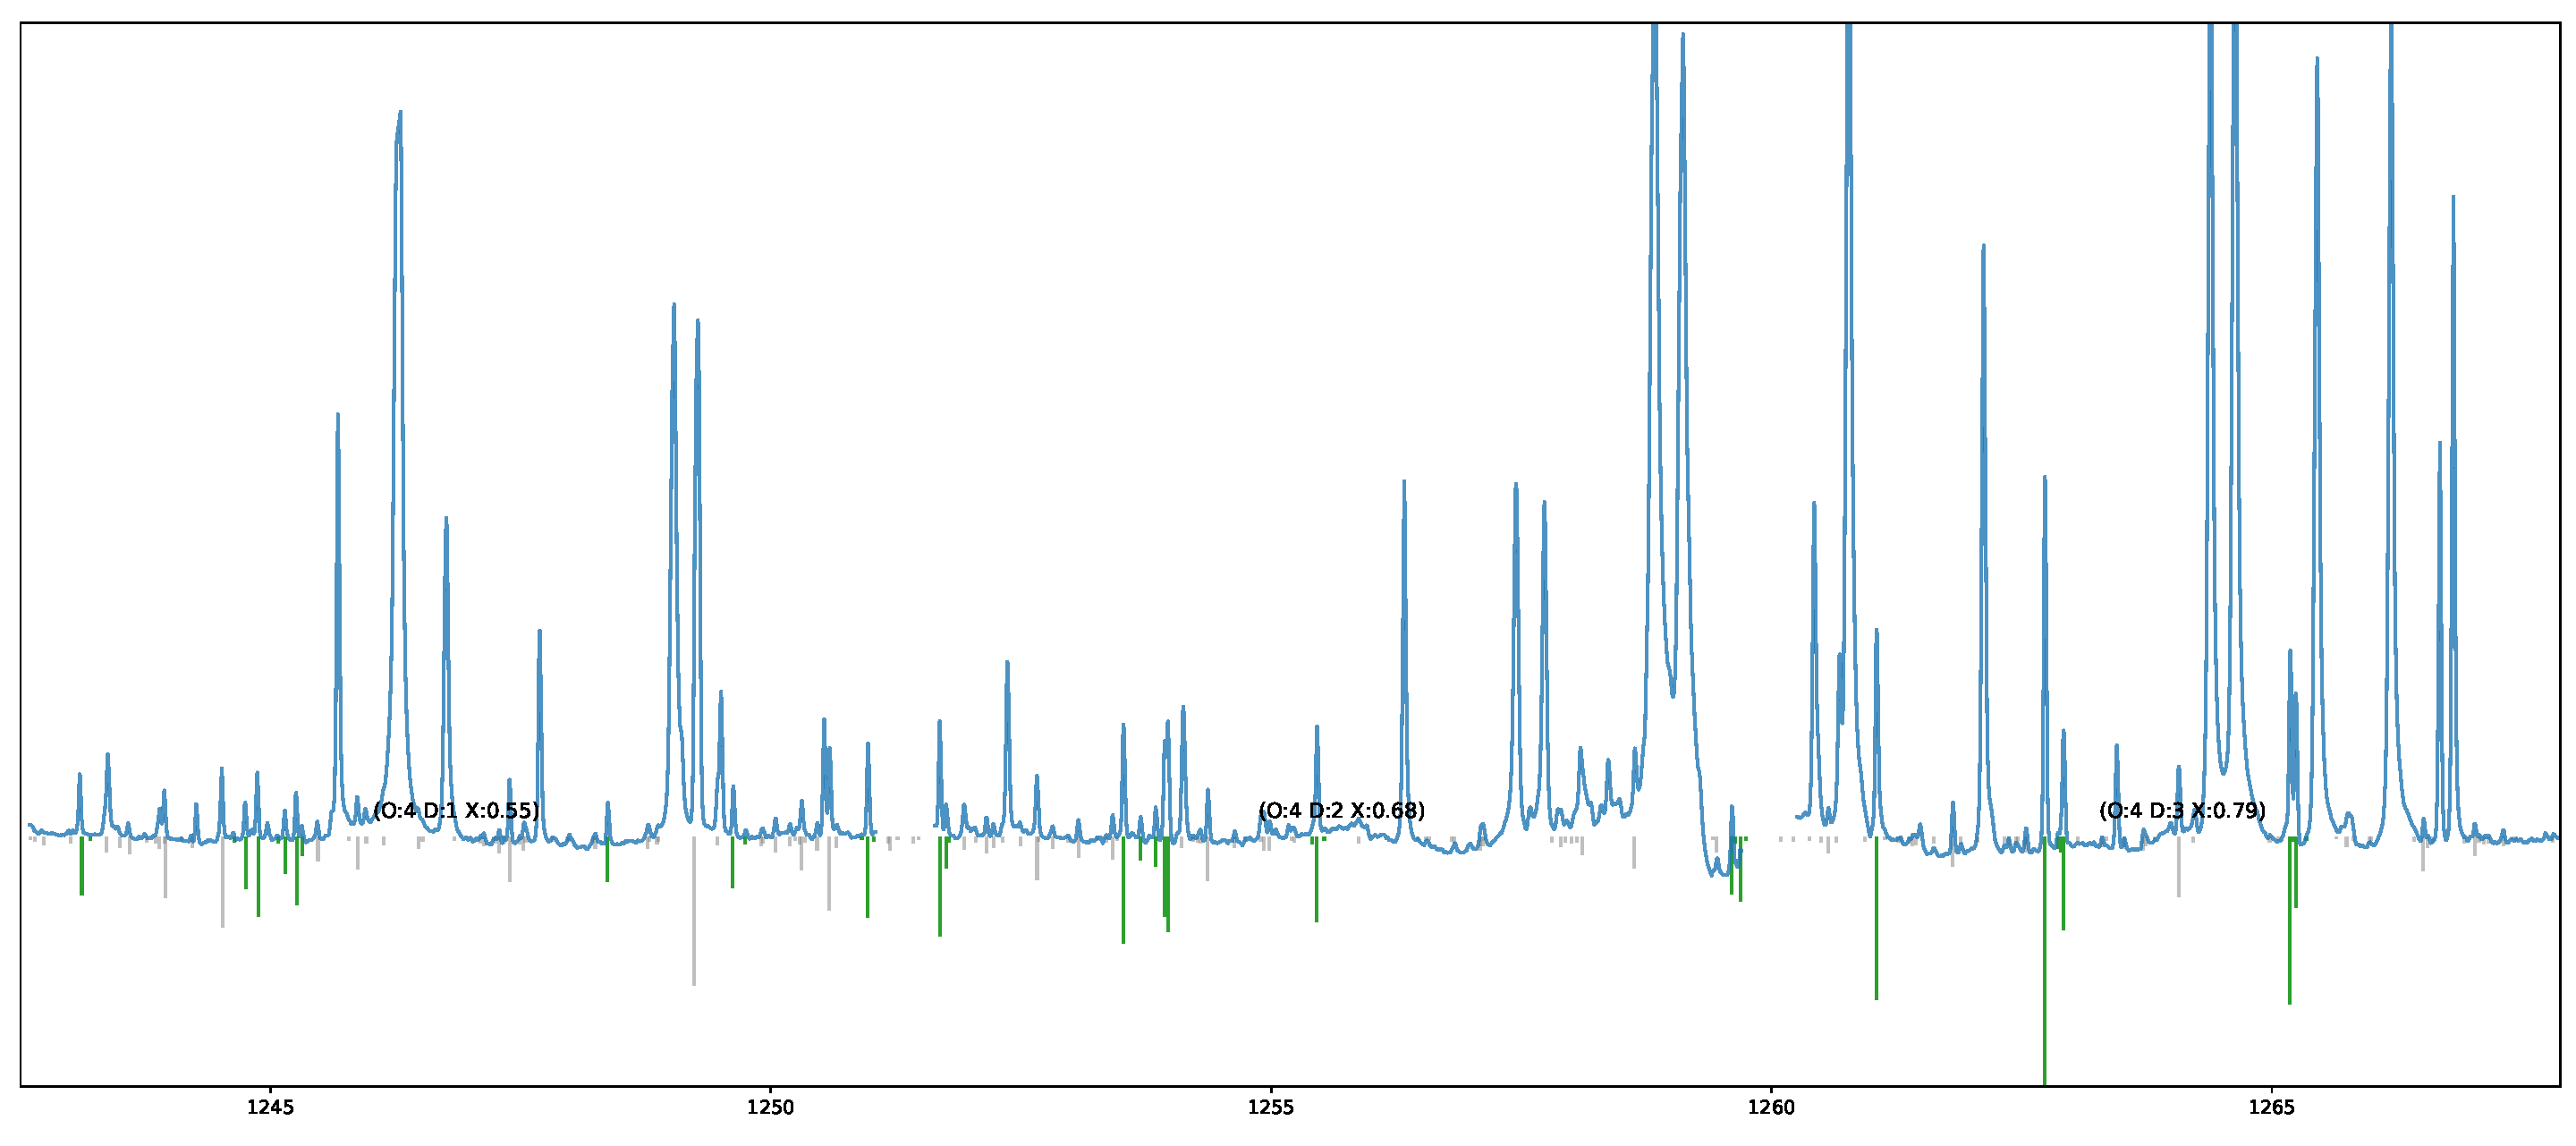
\includegraphics[width=1.25\linewidth, angle=90]{linesel_examp.pdf}
\end{center}
\caption{An example of a UNe spectrum in setting J1228. }
\label{fig:linesel}
\end{figure}


avoid blends
matching relative strength.

goal is cross-correlation
different selection needed for line-fitting.

\subsection{Wavelength calibration in L and M-bands}

Alexis' text (Oct 24 ?)

